\documentclass[11pt]{scrartcl}
\usepackage{dominatrix}
\usepackage{solarized-light}
\lstset{
language=python
}

\renewcommand\thesection{Problem \arabic{section}}
\renewcommand\thesubsection{\arabic{section} (\alph{subsection})}
\renewcommand\thesubsubsection{(\roman{subsubsection})}
\DeclareMathOperator{\AU}{AU}
\DeclareMathOperator{\arcsec}{arcsec}
\DeclareMathOperator{\pc}{pc}
\DeclareMathOperator{\km}{km}
\DeclareMathOperator{\m}{m}
\DeclareMathOperator{\cm}{cm}
\DeclareMathOperator{\rad}{rad}
\DeclareMathOperator{\s}{s}
\DeclareMathOperator{\degrees}{degrees}
\DeclareMathOperator{\degree}{degree}
\DeclareMathOperator{\arcmin}{arcmin}
\DeclareMathOperator{\parsec}{parsec}
\DeclareMathOperator{\lightyears}{light-years}

\newcommand\pow[2]{\ensuremath{#1 \times 10^{#2}}}

\title{Problem Set 1 Solutions}
\subject{ASTR 1404 Stars, Galaxies, and Cosmology}
%\author{James H. Applgate}
\begin{document}
\maketitle

\section{}

One full circle is $2\pi \rad$ and $360$ degrees. Thus the number of degrees in a $\rad$ is:

\[1\ \text{Circle} = 2\pi \rad = 360\degrees\]

Then,

\[1 \rad = \frac{360}{2\pi}\degrees\]

\subsection{}

\[1 \rad = 57.3\degrees\]

\subsection{}

\begin{align*}
1\degree &= 60\arcmin \\
1 \rad &= \frac{360}{2\pi} \degrees = \frac{360}{2\pi} \times 60 \arcmin \\
1 \rad &= \pow{3.44}{3}\arcmin
\end{align*}

\subsection{}

\begin{align*}
1\arcmin &= 60\arcsec \\
1 \rad &= \pow{3.44}{3}\arcmin = (\pow{3.44}{3})\times(60)\arcsec \\
1 \rad &= \pow{2.06}{5}\arcsec
\end{align*}

\subsection{}

\begin{align*}
1 \degree &= \frac{2\pi}{360}\rad \\
1 \degree &= 0.0175 \rad = {1.75}{-2}\rad
\end{align*}

\subsection{}

\begin{align*}
1 \arcmin &= \frac{1}{60}\deg \\
1 \arcmin &= \frac{2\pi}{360} \times \frac{1}{60} \rad \\
1 \arcmin &= \pow{2.91}{-4}\rad
\end{align*}

\subsection{}

\begin{align*}
1 \arcmin &= \pow{2.91}{-4}\rad \\
1 \arcsec &= \frac{1}{60}\arcmin = \pow{2.91}{-4} \times \left(\frac{1}{60}\right) \rad \\
1 \arcsec &= \pow{4.85}{06}\rad
\end{align*}


\section{}

The angular separation of the Earth-Moon system as seen from the Sun is

\begin{align*}
\theta &=\frac{\text{Earth-Moon distance}}{1\AU} \\
&= \frac{\pow{3.84}{10}\cm}{\pow{1.5}{13}\cm} \\
&= \pow{2.56}{-3}\rad \\
&= 0.147 \degrees = 8.8\arcmin
\end{align*}

Remember that $1\AU = \pow{1.5}{13}\cm$ and $D_M = 384,000\km = \pow{3.84}{10}\cm$


\section{}

\subsection{}

\begin{align*}
\theta_J &= \frac{D_J}{4\AU} \\
&= \frac{\pow{1.43}{10}\cm}{\pow{6}{13}\cm} = \ \text{Angular diameter of Jupiter} \\
&= \pow{2.38}{-4}\rad = \pow{1.73}{-2}\degrees \\
&= 0.82 \arcmin = 49\arcsec
\end{align*}

\subsection{}

A human with 20/20 vision can resolve about one $\arcmin$, so Jupiter is a bit too small for us to see as a disk on the sky. It is pretty easy to resolve with a small telescope. See the attached drawings by Galileo and others from 1610.

\begin{figure}[H]
\centering
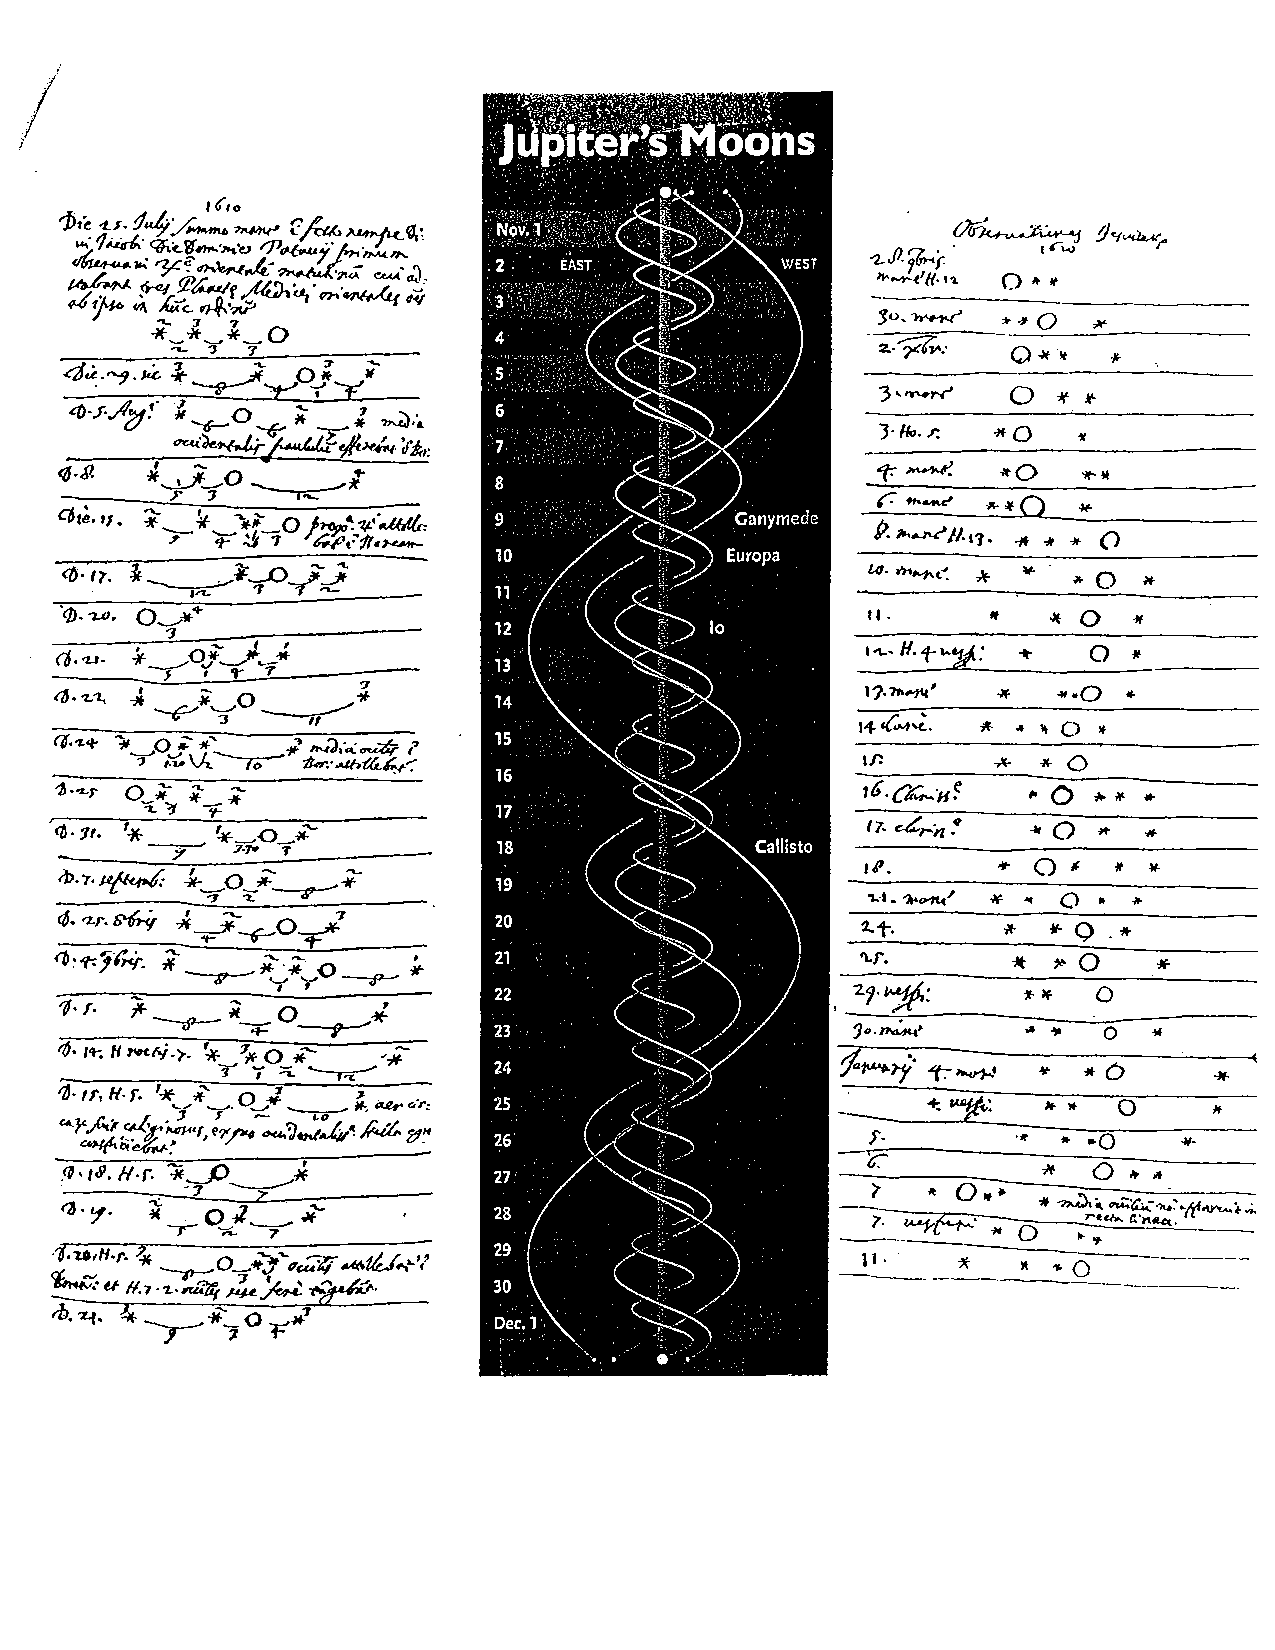
\includegraphics[width=\textwidth]{figures/problem-set-1-galileo-drawings.pdf}
\caption{Galileo's drawings of Jupiter and its satellites}
\end{figure}


\section{}

\begin{figure}[H]
\centering
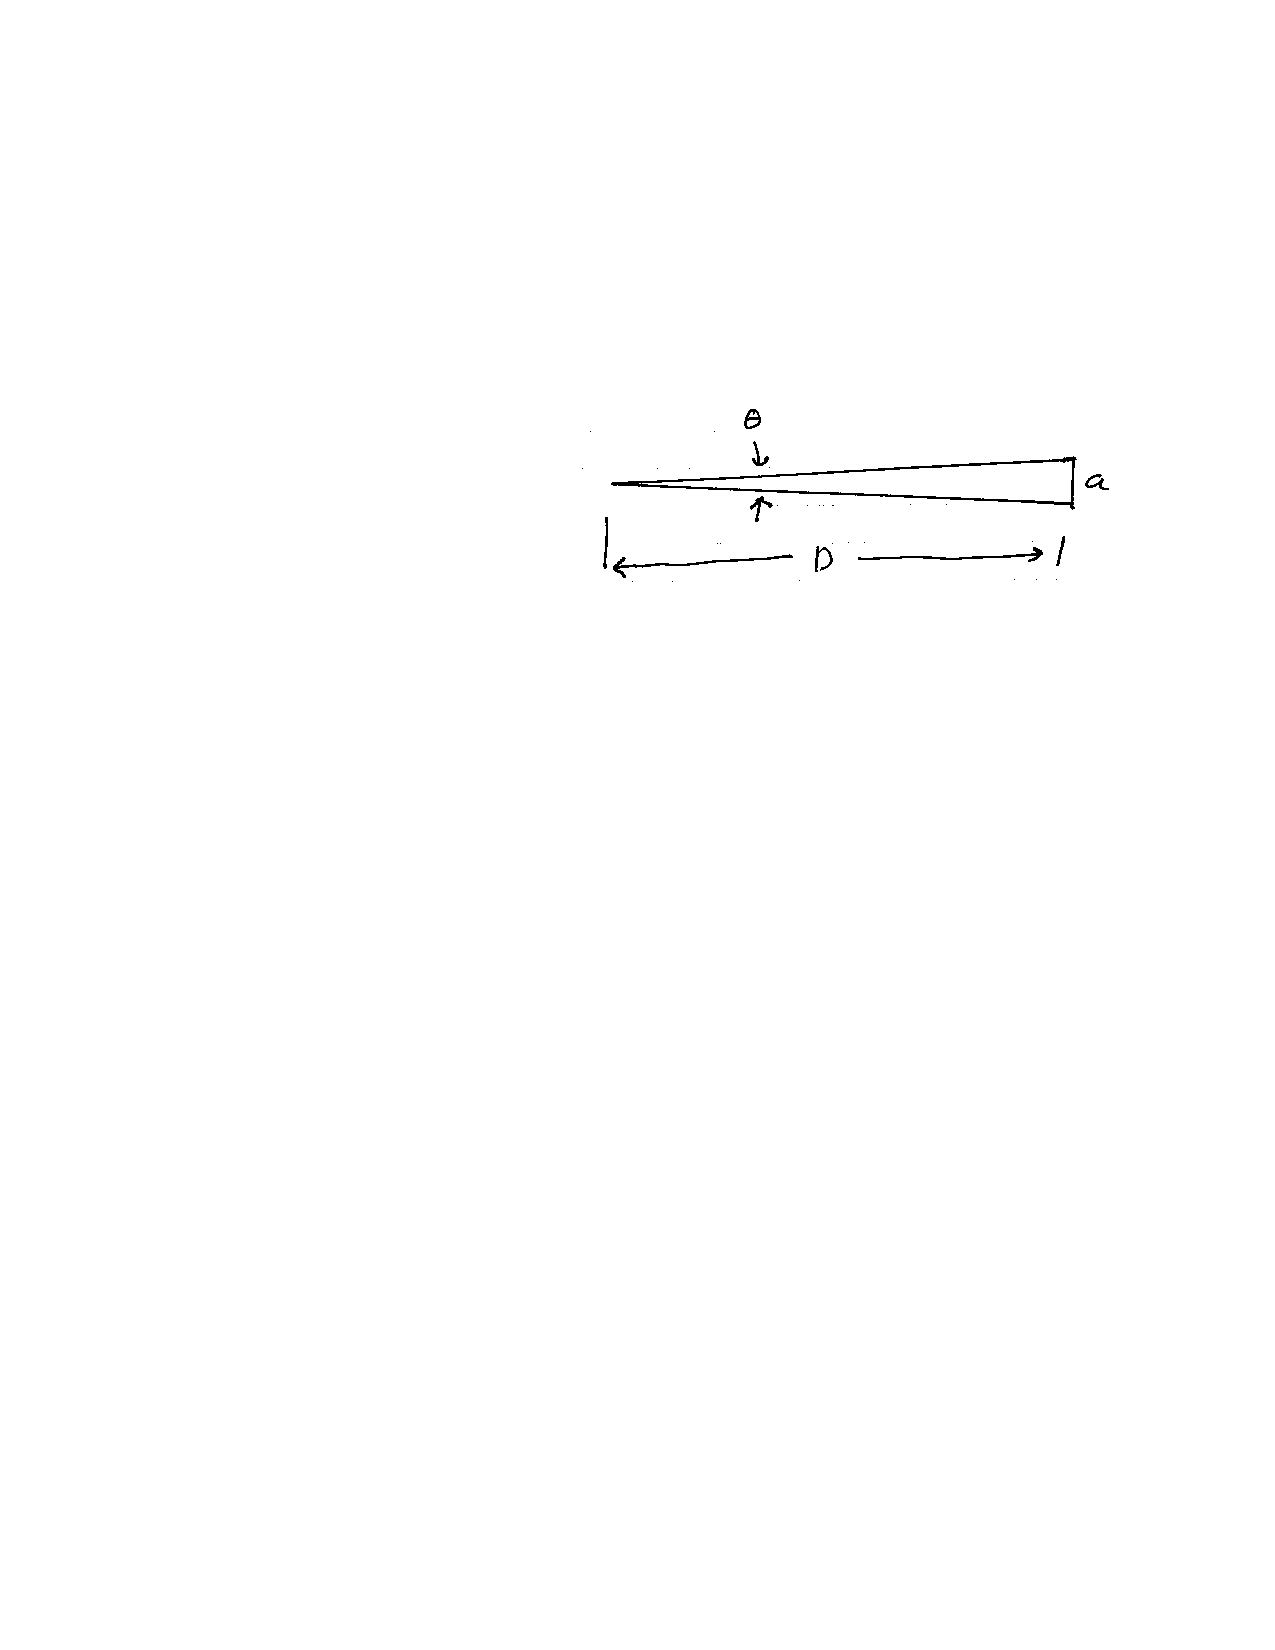
\includegraphics[width=\textwidth]{figures/problem-set-1-skinny-triangle-hand.pdf}
\caption{Law of Skinny Triangles where $a = \theta \cdot D$.}
\end{figure}

Law of Skinny Triangles: $a = \theta \cdot D$. Here,

\begin{itemize}
\item $a =\ \text{Short Side} = \ \text{Diameter (physical of Saturn's rings)}$
\item $D = \ \text{Long Side} = \ \text{Distance to Saturn}$
\item $\theta = \ \text{Small angle (in rad)}$
\end{itemize}

Convert $\theta$ to radians:

\[\theta = 39\arcsec = \left(\pow{4.85}{-6}\frac{\rad}{\arcsec}\right) = \pow{1.89}{-4}\rad\]

\[D = \pow{1.3}{14}\cm = \ \text{Distance to Saturn}\]

Diameter of rings = $\theta \times D$ = $\left(\pow{1.89}{-4}\right) \times \left(\pow{1.3}{14}\right) \cm = a$. Then, $a = \pow{2.46}{10}\cm = 246,000\km$.


\section{}

The Law of Skinny Triangles is $a = \theta D$. Here the short side is the baseline of the two observers on Earth.

\begin{align*}
a &= R_E = \pow{6.37}{8}\cm = \ \text{Radius of Earth} \\
\theta &= 31.3 \arcsec = \pow{1.52}{-4} \rad \\
D &= 0.28\AU = \ \text{Earth-Venus distance at Transit}
\end{align*}

This gets

\begin{align*}
D &= \frac{R_E}{\theta} = \frac{\pow{6.37}{8}\cm}{\pow{1.52}{-4}} = \pow{4.2}{12}\cm \\
&= 0.28\AU
\end{align*}

This implies that $1\AU = \frac{\pow{4.2}{12}\cm}{0.28} = \pow{1.50}{13}\cm$


\section{}

We have $a = \theta D$ where $a$ is the separation of $19,600\km$ and $D$ is $40\AU = \pow{6}{14}\cm$. Then $\theta = \frac{a}{D}$

\[\theta = \frac{\pow{1.96}{9}\cm}{\pow{6}{14}\cm} = \pow{3.27}{-6}\rad = 0.67\arcsec\]

The Pluto-Charon separation is barely resolvable from the ground. The resolution of a ground based telescope is a bit less than one arcsecond due to the distortion of images produced by the atmosphere. Note: The image in Figure \ref{fig-problem-set-1-pluto-charon}, first recorded in 1978, resulted in Pluto's eventual fall from ``Planet'' status.

\begin{figure}[H]
\centering
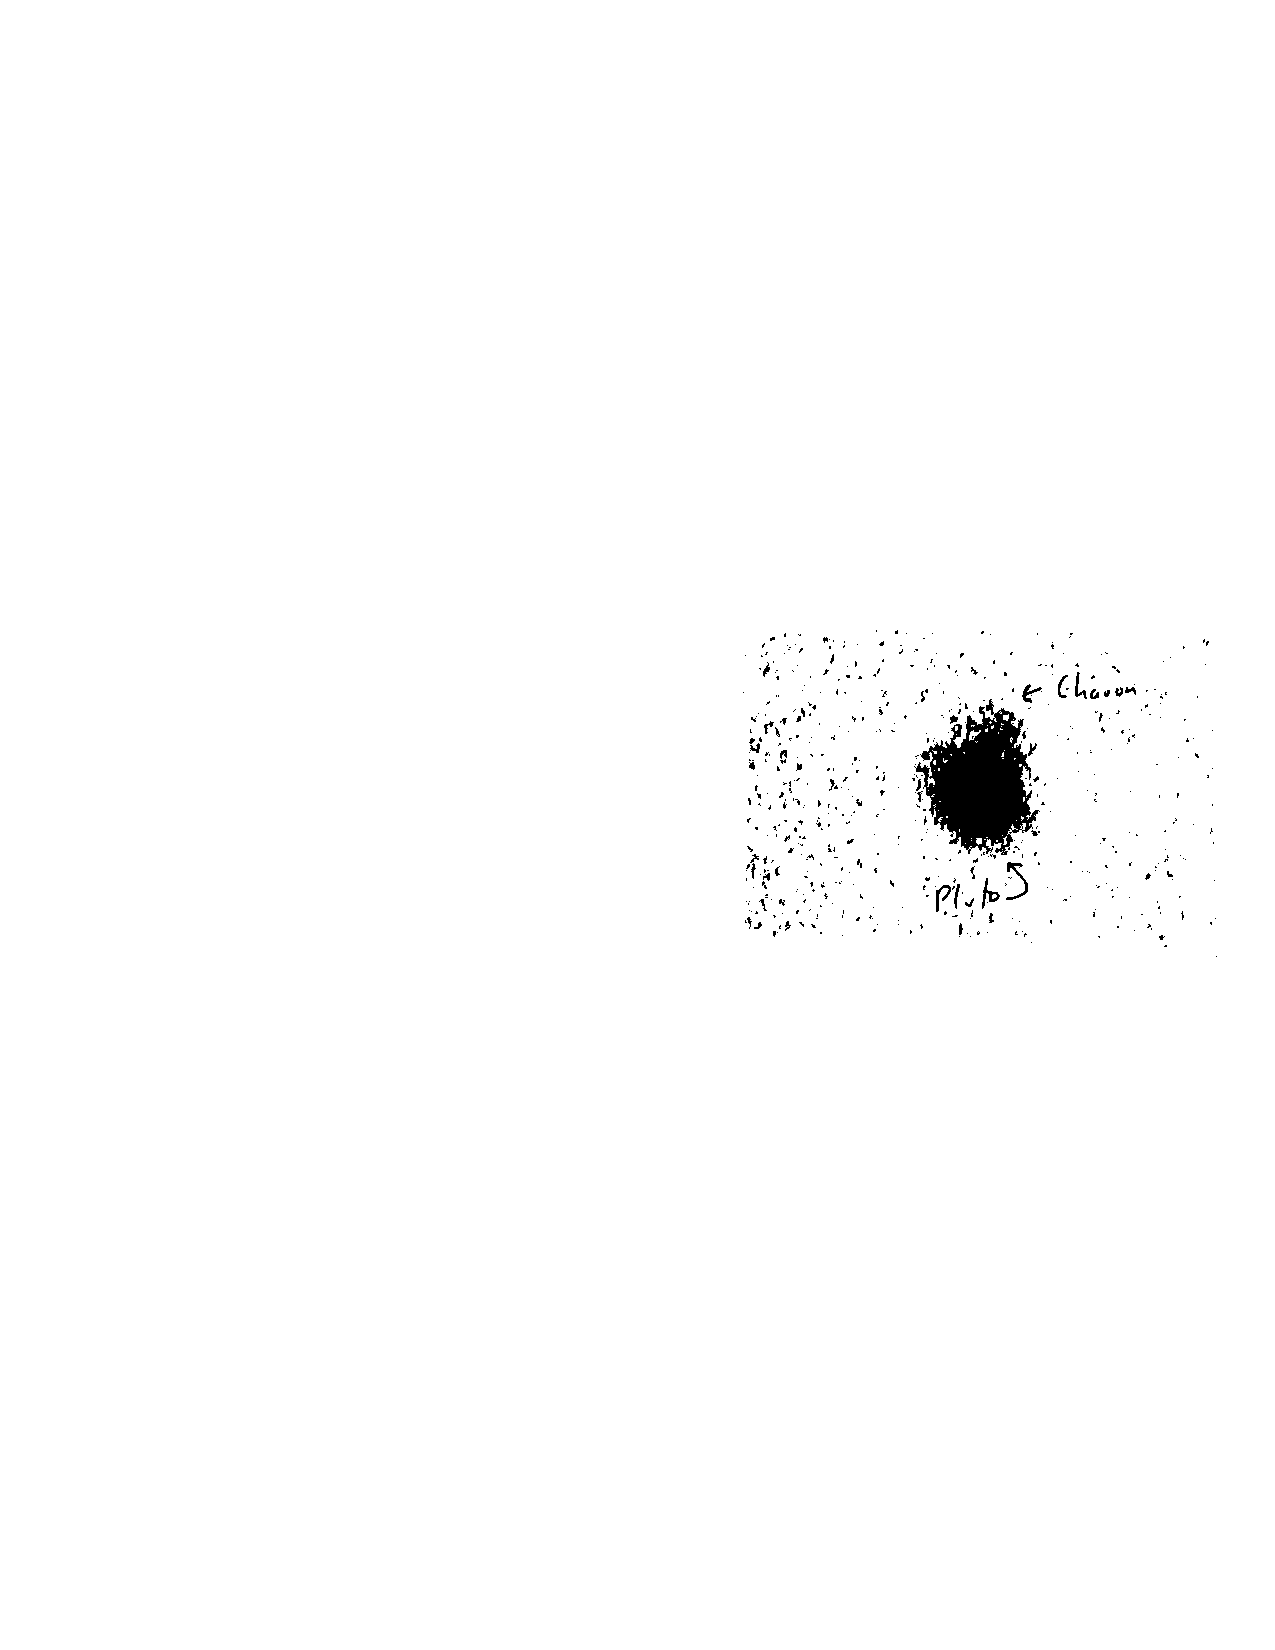
\includegraphics[width=0.5\textwidth]{figures/problem-set-1-pluto-charon.pdf}
\caption{Highly enlarged image of Pluto on photograph made at the U.S. Naval Observatory, Flagstaff Station. The ``bump'' on the upper right is Pluto's satellite, Charon. (Courtesy, U.S. Naval Observatory)}
\label{fig-problem-set-1-pluto-charon}
\end{figure}


\section{}

The angular separation of the satellite and the center of Jupiter's dish is given by

\[\theta = \frac{a}{D}\]

where $a = \ \text{Moon-Jupiter Separation}$, $D = \ \text{Earth-Jupiter Distance} = \pow{6}{13}\cm$

\begin{table}[H]
\centering
\begin{tabular}{c c c}
\toprule
Moon & Moon Jupiter Distance & $\theta$ \\
\midrule
Io & $\pow{4.22}{10}\cm$ & $\pow{7.03}{-4}\rad = 2.42\arcmin$ \\
Europa & $\pow{6.71}{10}\cm$ & $\pow{1.21}{-3}\rad = 3.84\arcmin$ \\
Ganymede & $\pow{1.07}{11}\cm$ & $\pow{1.78}{-3}\rad = 6.13\arcmin$ \\
Callisto & $\pow{1.88}{11}\cm$ & $\pow{3.13}{-3}\rad = 10.8\arcmin$ \\
\bottomrule
\end{tabular}
\caption{Angular separations ($\theta$) of Jupiter's moons and the center of Jupiter's dish.}
\end{table}


\section{}

The law of skinny triangles may be written 

\[a = \theta D\]

with $a$, $D$ in the same distance units and $\theta$ in radians. The definition of the parsec allows us to write it in the form

\[a(\AU) = \theta(\arcsec) \cdot D (\parsec)\]

The definition of a parsec, a length of $1\AU$ subtends an angle of $\arcsec$ if viewed from a distance of $1 \parsec$, is clearly expressed by this relation.

\begin{align*}
a(\AU) &= \ \text{short side expressed in AU} \\
\theta &= \ \text{Small angle expressed in arcseconds} \\
D(\parsec) &= \ \text{Long side in parsecs}
\end{align*}

Conversion factors are:

\begin{align*}
1 \parsec &= \pow{2.06}{5}\AU \\
&= \pow{3.09}{18}\cm = \pow{3.09}{16}\m \\
&= 3.26 \lightyears
\end{align*}

For stellar parallax observed from Earth, $a(\AU) = 1$, so $D(\parsec) = \frac{1}{\theta(\arcsec)}$.


\subsection{}

\[\theta = 0.37\arcsec \ \text{for Sirius}\]

Then,

\[D(\parsec) = \frac{1}{0.37} = 2.7\parsec\]

\subsection{}

\[D(\cm) = \pow{3.09}{18}\cm \cdot D(\parsec) = \pow{8.35}{18}\cm = \pow{8.35}{16}\m\]

\subsection{}

\[D(\lightyears) = 3.26D(\parsec) = 8.8\lightyears\]


\section{}

\subsection{}

Distance to $\alpha$Cen in $\parsec$ is $D(\parsec) = \frac{1}{\text{parallax in arcsec}} = \frac{1}{0.75}\parsec = 1.33\parsec$.

\subsection{}

\[\theta = \frac{a(\AU)}{D(\parsec)} = \frac{5.2}{1.33} = 3.9\arcsec\]

\end{document}
